\documentclass[tikz, border=10pt]{standalone}
\usepackage{pgfplots}
\pgfplotsset{compat=1.17}
\usepackage{pgfmath} % Para cálculos matemáticos
\begin{document}

% Definición de la macro para generar una curva con proceso AR(1)
\newcommand{\plotARcurve}[2]{%
    % #1: Semilla (número entero) para la aleatoriedad
    % #2: Color de la curva
    \pgfmathsetseed{#1}%
    % Generar valor inicial para AR (entre -0.3 y 0.3)
    \pgfmathsetmacro{\AR}{(rand - 0.5)*0.6}%
    % Crear la lista de coordenadas
    \def\coordlist{(1, {0.5*exp(0.25*1)*(1+\AR)})}%
    \foreach \x in {2,...,14} {%
       % Generar perturbación epsilon en el intervalo aproximado [-0.3,0.3]
       \pgfmathsetmacro{\noise}{(rand - 0.5)*0.6}%
       % Actualizar el proceso AR: AR(n) = 0.8 * AR(n-1) + noise
       \pgfmathsetmacro{\AR}{0.8*\AR + \noise}%
       % Agregar la coordenada para el día \x
       \xdef\tempcoord{(\x, {0.5*exp(0.25*\x)*(1+\AR)})}%
       \xdef\coordlist{\coordlist \space \tempcoord}%
    }%
    % Graficar la curva con la lista de coordenadas generada
    \addplot[mark=*, mark size=1.5pt, color=#2, thick] coordinates {\coordlist};%
}

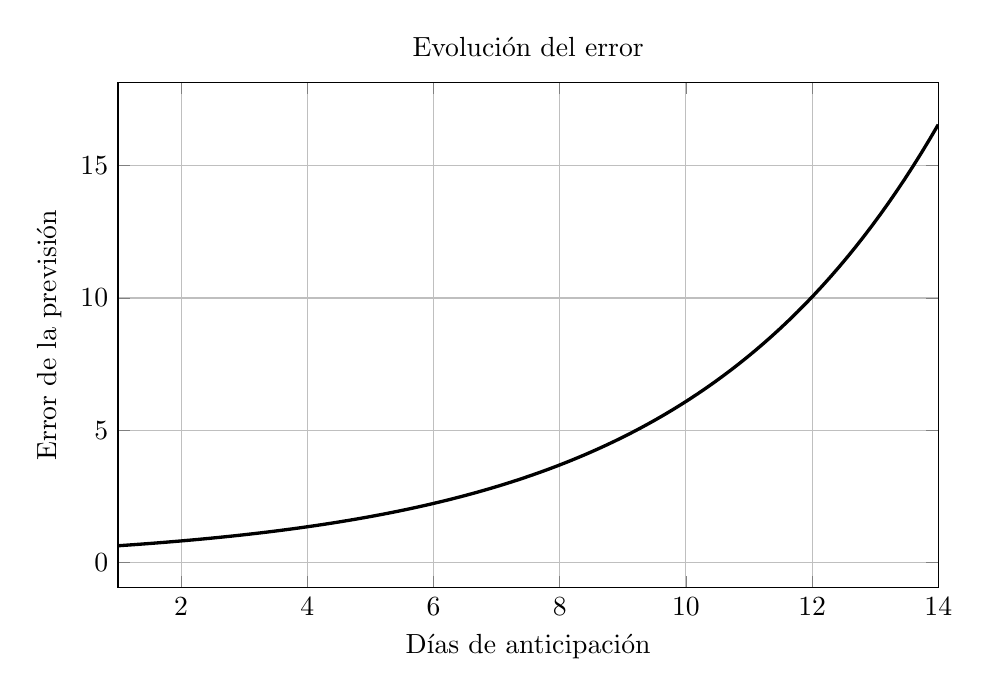
\begin{tikzpicture}
  \begin{axis}[
      xlabel={Días de anticipación},
      ylabel={Error de la previsión},
      xmin=1, xmax=14,
      grid=both,
      title={Evolución del error },
      width=12cm, height=8cm,
      legend pos=north west,
    ]
    
    % Se generan 15 curvas, cada una con distinta semilla y color
    \plotARcurve{1}{red}
    \plotARcurve{2}{blue}
    \plotARcurve{3}{green}
    \plotARcurve{4}{orange}
    \plotARcurve{5}{violet}
    \plotARcurve{6}{cyan}
    \plotARcurve{7}{magenta}
    \plotARcurve{8}{teal}
    \plotARcurve{9}{brown}
    \plotARcurve{10}{black}
    \plotARcurve{11}{olive}
    \plotARcurve{12}{lime}
    \plotARcurve{13}{pink}
    \plotARcurve{14}{purple}
    \plotARcurve{15}{gray}
    
    % Se dibuja la curva de tendencia media (sin la componente AR)
    \addplot[
      domain=1:14,
      samples=100,
      very thick,
      color=black,
    ] {0.5*exp(0.25*x)};

    
  \end{axis}
\end{tikzpicture}
\end{document}
